\documentclass[]{IEEEphot}

% Fix for undefined bold font shape
\usepackage{lmodern}
\renewcommand{\bfdefault}{bx}

\jvol{1}
\jnum{1}
\jmonth{March}
\pubyear{2025}

\newtheorem{theorem}{Theorem}
\newtheorem{lemma}{Lemma}

\usepackage{listings}

\begin{document}

\title{Final Project Report}

\author{
    Team\#11 (Option 3):\\
    Chou, Kelvin, 862466579\\
    Yu, Kunyi, 862548836\\
    Ibrahim, Mona, 862267986
}

\maketitle

\markboth{CS225 Spatial Computing}{Final Project Report (option 3)}

\begin{abstract}
    This report focuses on the code and experiment replication of the provided paper \cite{ref1-original-paper} and corresponds to project option 3. It begins with a paper review, covering the summary of query problems, indexing architecture, and the POWER query processing algorithm. Next, the code replication process is introduced, including code decomposition and experiment design. Finally, the experiment results are presented and discussed, followed by the conclusion.
\end{abstract}

\begin{IEEEkeywords}
    kNN spatial-keyword query, Indexing architecture, Query processing algorithm, Code replication
\end{IEEEkeywords}

\section{Paper Review}

The paper of cutting-edge Spatial-keyword querying process is a 2022 published paper by Yongyi Liu and Amr Magdy \cite{ref1-original-paper}. Main contributions of the paper includes:

\begin{enumerate}
    \item Propose two novel kNN spatial-keyword query problems
          \begin{itemize}
              \item TKQN: Top-k kNN Query with Negative keyword predicates (we choose this)
              \item BKQN: Boolean kNN Query with negative keyword predicates
          \end{itemize}
    \item Introduce U-ASK: a unified architecture for spatial-keyword query with negative keyword predictions
    \item Introduce POWER: a query processing algorithm handling TKQN and BKQN queries
    \item Present experimental evaluation on real datasets
\end{enumerate}

Current work of the spatial-keyword querying process has two limitations: one is lack of dealing with phrases with a sequence of words, and the other one supports only boolean kNN query. To handle the limitations, U-ASK proposed by the paper supports two types of kNN spatial-keyword queries with AND, OR, and NOT conjunctions, which consists of an index framework TEQ (Textual Enhanced Quadtree) and a query processing algorithm POWER (Parallel Bottom-up Search with Incremental Pruning).

The problem of TKQN takes a tuple of location, positive/negative keywords, weight factor, and number k, then outputs top-k output with at least one positive keyword, without any negative keyword, and ranked by a spatial-textual-score function. The input format is as follows:

$$q_t = (q_t.loc, q_t.pos, q_t.neg, q_t.\lambda, q_t.k)$$

The score function is defined as:

$$score(o_i, q_t) = q_t.\lambda * score_s(o_i, q_t) + (1 - q_t.\lambda) * score_t(o_i, q_t)$$

Moreover, TEQ indexing is a hybrid, memory-resident index for TKQN queries which combines the strengths of a quadtree for spatial partitioning and an inverted index for keyword organization. Structure: each leaf cell $n$ in the quadtree contains 4 components:

\begin{enumerate}
    \item $n.ltp$: a location table pointer to a hash file on disk
    \item $n.neigh$: a list of spatial neighboring cells
    \item $n.iti$: an inverted textual index (hashtable) mapping keyword $w$ to the tuple:
          \begin{enumerate}
              \item $w.size$: number of objects containing the keyword $w$
              \item $w.max$: maximum weight of $w$ in the cell
              \item $w.listPtr$: pointer to the sorted inverted list file
              \item $w.setPtr$: pointer to the sorted inverted set file (faster boolean filtering)
          \end{enumerate}
    \item $n.oti$: an object textual index (hashtable) mapping object IDs to full text
\end{enumerate}

The way of constructing TEQ contains two passes. The first pass builds the spatial indexing component: (build tree)

\begin{enumerate}
    \item Insert objects into the quadtree
    \item Quadtree cells are split based on object density
    \item Create $n.neigh$ and $n.ltp$
\end{enumerate}

The second pass builds the textual indexing component: (build cells)

\begin{enumerate}
    \item Initialize two hashtables: $n.iti$ and $n.oti$
    \item Insert every object $o$ into $n.oti$
    \item Insert every keyword $w$ with its weight into $n.iti$
    \item Sort inverted list and inverted set, store all parameters into disk
\end{enumerate}

The query problem our group chose is TKQN, so as requirements, we need to implement the POWER algorithm. The POWER (Parallel bOttom-up search With incrEmental pRuning) operates within a master-worker framework, where each worker processes local top-k searches within assigned index cells. First, the POWER will process index cell by loading location table $n.LT$ into a buffer with LRU policy (prepared for parallelization, the project will omit it). Second, the POWER uses a top-k search strategy based on the Threshold Algorithm (TA), which incrementally retrieves and aggregates scores from multiple sorted lists. Thanks to the upper bound score, it will prune many useless searches. Third, because the TKQN query ranks its results based on textual attribute (can be found in keyword-inverted lists) and spatial attribute (sorted based on the query location), a priority queue will incrementally retrieve top-k objects based on the TA algorithm mentioned before. Lastly, the POWER will evaluate both positive keyword predictions ($q.pos$) and negative keyword predictions ($q.neg$) by a series rigorous steps. Note that, due to the computationally expensive nature of using a priority queue, the paper also introduces POWER-T (textual pruning) and POWER-S (spatial-pruning) to reduce query cost, but the project option 3 will not cover this part.

The experimental evaluation is in section 6 of the paper, which contains 6.1) experimental setup, 6.2) performance evaluation for the different parameters and framework components, and 6.3/4) compares the proposed algorithms against the SOTA under TKQN and BKQN, respectively. In addition to 6.1) experimental setup, the experiments suitable for this project are mainly distributed in 6.3) TKQN query evaluation.

For the 6.1) experimental setup, there is a summary in the “Table 2: Evaluation Parameters Values” of the paper.

For the 6.3) TKQN query evaluation, 4 experiments are conducted:

\begin{enumerate}
    \item The effect of query keywords: change different number of positive words ($|q.pos|$), number of negative phrases ($|q.neg|$), and length of negative phrases ($q.negLen$), showing how the performance floats;
    \item The effect of weighting factor: change different weighting factors ($\lambda$), showing how the balance between spatial and textual scores affects performance;
    \item The effect of $k$: change different answer sizes ($q.k$), showing how the multi-threading master-worker architecture of POWER-T affects;
    \item The effect of dataset size: change different dataset sizes, showing how the scalability varies.
\end{enumerate}

The figures of above experiments’ results can be found in the “Figure 5: TKQN Query Evaluation” of the paper.

\section{Code Replication}

In our code replication process, we choose Python as programming language and manage with multi files to decompose the complexity of the project. The python source files are stored in directory $./src$ and the structure is as follows:

\begin{lstlisting}
    ./src
    ├── exps
    │   ├── exp_a.py
    │   ├── exp_b.py
    │   ├── exp_c.py  // deprecated, not applicable for POWER_batch
    │   ├── exp_d.py  // deprecated, no lambda for POWER/POWER_batch
    │   ├── exp_e.py
    │   └── exp_f.py
    ├── invertedIndex.py
    ├── main.py
    ├── plots.py
    ├── point.py
    ├── power.py
    ├── power_batch.py
    ├── quadTreeNode.py
    ├── query.py
    └── read_data.py
\end{lstlisting}

The main entry of the project is $main.py$, which contains the main function to run the experiments. The $read\_data.py$, $point.py$, $quadTreeNode.py$, $invertedIndex.py$, $query.py$, $power.py$, and $power\_batch.py$ are the core modules of the project. The implementation logic are follow the paper closely. Note that the $power_batch.py$ is used to run the experiments in batch mode, which will first gether the queries with the same parameters into a group and then run the POWER algorithm for each group.

The $plots.py$ is used to generate the plots for the experiments. The $exps$ directory contains the experiments mentioned in the paper subsection 6.3. The python files in the $exps$ directory will be called by the $main.py$ to run the experiments.

Instruction to run the code:

\begin{lstlisting}
    $ python main.py --exp=<exp_name> --size=<dataset_size>
    $ # exp_name: a, b, c, d, e, f (default a)
    $ # dataset_size: 2, 4, 6, 8, 10 (default 4)
\end{lstlisting}

For the data input, we use the class provided one and rename it as $./data$ directory. The data files are not included in the submission code due to the size limitation.

\newpage

\section{Experiment Results}

The parameters settings for the experiments are remained the same as the paper. You may find those parameters in the $./src/exps/$ directory and $./src/main.py$ which are well commented. The following table shows the details which is copied from the paper\cite{ref1-original-paper}, default settings use \textbf{bold} font format:

\begin{figure}[h]
    \centering
    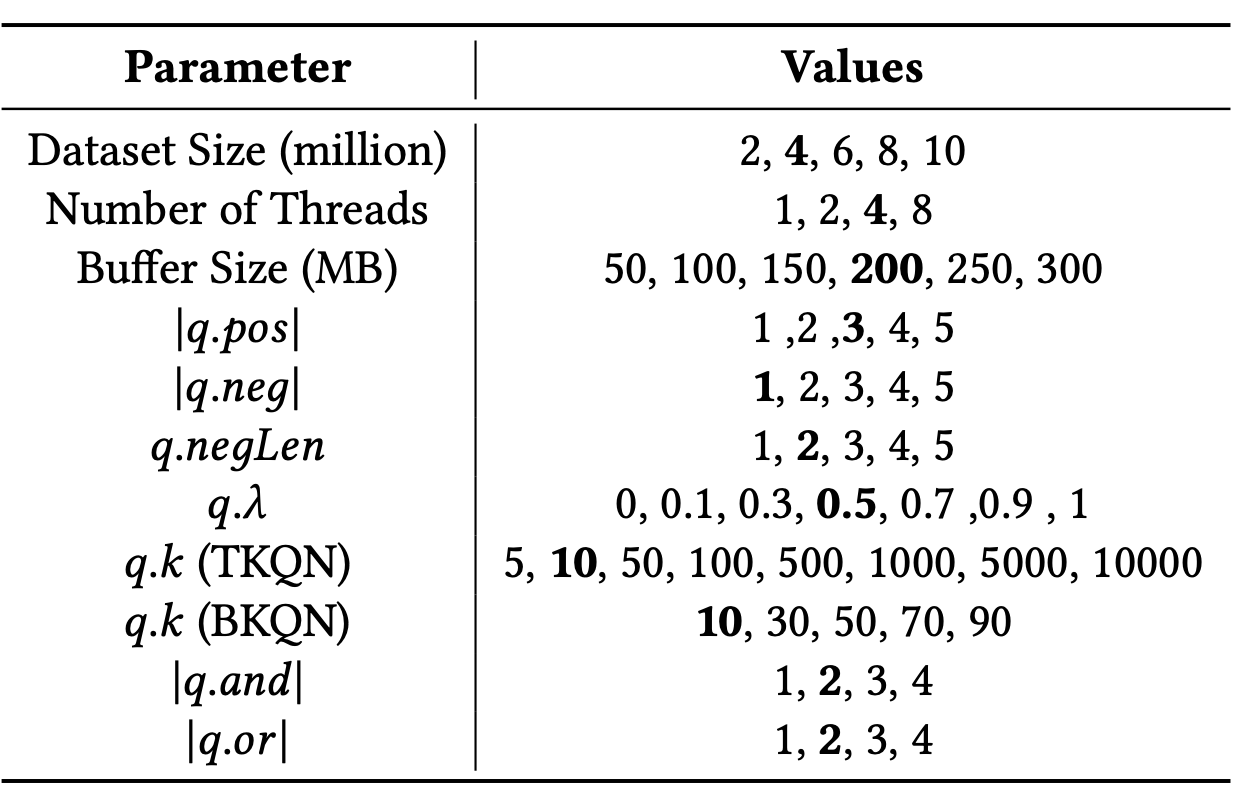
\includegraphics[width=0.6\textwidth]{pics/exp_settings.png}
\end{figure}

Note that all experiments use 50 queries from the dataset.

In the paper, there are 6 experiments (a/b/c/d/e/f) conducted related to TKQN query evaluation. Among them, we have successfully replicated the experiments a, b, c, e, and f. Because the weighting factor $\lambda$ is not presented in the POWER algorithm, experiment d is deprecated. The following parts will show the results of these experiments separately.

\subsection{Experiment a}

The purpose of experiment a is to evaluate the effect of changing the number of positive words to the performance of query latency (runtime).

\begin{figure}[h]
    \centering
    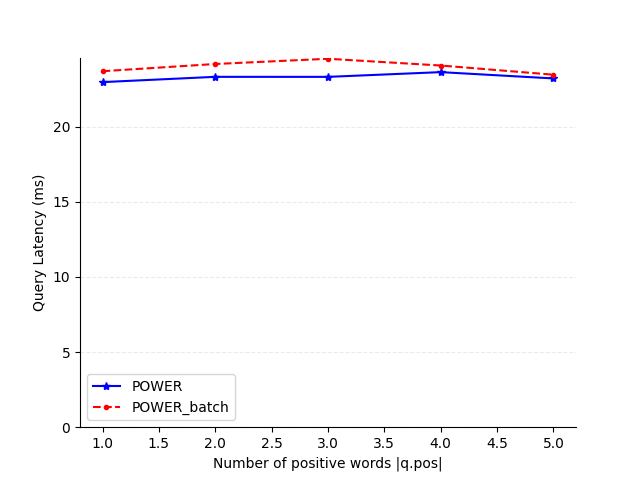
\includegraphics[width=0.4\textwidth]{../exp_plots/a_4m_50queries_20250314-212142.png}
    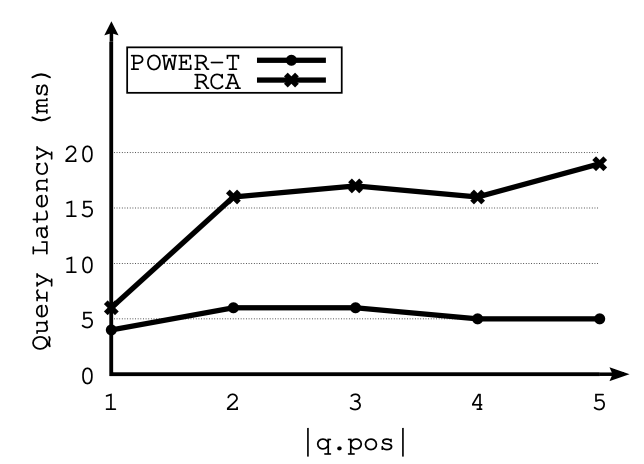
\includegraphics[width=0.4\textwidth]{./pics/paper-exp-a.png}
    \caption{Comparison of experiment a, left: our result, right: paper result}
\end{figure}

The left figure (our result) shows that the runtime of the POWER and POWER\_batch algorithms barely changes (around 11ms) with different numbers of positive words. The result is similar to the right figure (paper result) where the query latency is stable at 5ms. The reason for the difference in the runtime maybe due to the different hardwares and implementation languages.

\subsection{Experiment b}

The purpose of experiment b is to evaluate the effect of changing the number of negative phrases to the performance of query latency (runtime).

\begin{figure}[h]
    \centering
    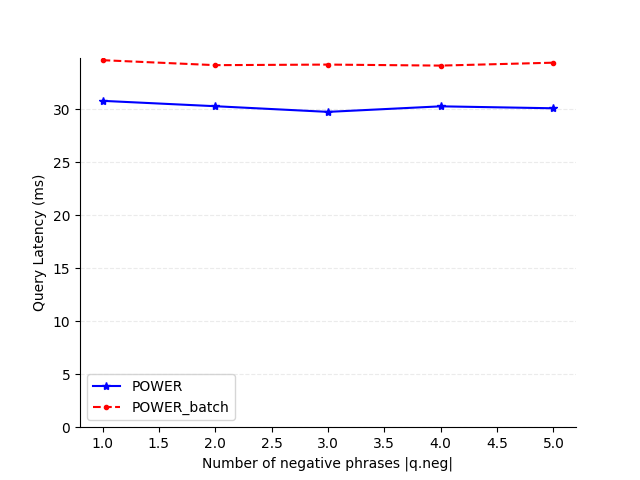
\includegraphics[width=0.4\textwidth]{../exp_plots/b_4m_50queries_20250314-212603.png}
    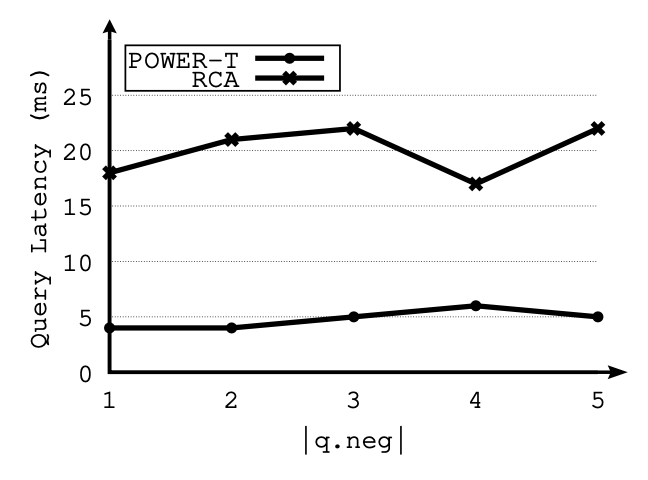
\includegraphics[width=0.4\textwidth]{./pics/paper-exp-b.png}
    \caption{Comparison of experiment b, left: our result, right: paper result}
\end{figure}

The left figure (our result) yields a great result that the runtime of both POWER and POWER\_batch algorithms stay stable at around 33ms with different numbers of negative phrases. The batch version has a slightly higher runtime than the single version, may be due to the overhead of gathering queries. The right figure (paper result) shows that the runtime is stable at 5ms for all negative phrase numbers. The runtime difference may be due to the different hardwares and implementation languages.

\subsection{Experiment c - Deprecated}

The purpose of experiment c is to evaluate the effect of length of negative phrases to the performance of query latency (runtime). But the experiment c is not applicable for the POWER\_batch algorithm.

\subsection{Experiment d - Deprecated}

The experiment d is deprecated because the weighting factor $\lambda$ is not presented in the POWER algorithm.

\subsection{Experiment e}

The purpose of experiment e is to evaluate the effect of changing the parameter $k$ (in kNN) to the performance of query latency (runtime).

\begin{figure}[h]
    \centering
    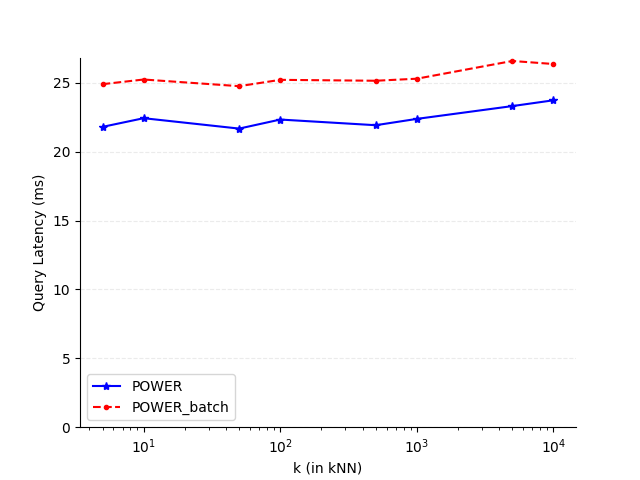
\includegraphics[width=0.4\textwidth]{../exp_plots/e_4m_50queries_20250314-214212.png}
    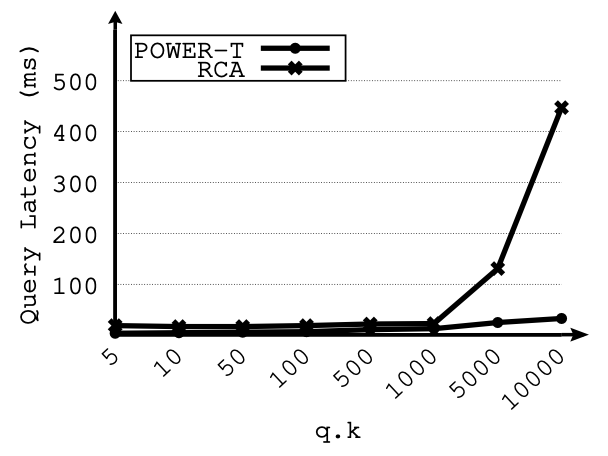
\includegraphics[width=0.4\textwidth]{./pics/paper-exp-e.png}
    \caption{Comparison of experiment e, left: our result, right: paper result}
\end{figure}

The left figure (our result) shows that the runtime of the POWER and POWER\_batch algorithms remains stable at around 23ms with different values of $k$. At the same time the right figure (paper result) shows that the runtime is in a exponential growth trend with the increase of $k$. May be the reason for the difference is our implementation uses a small dataset size (4m) which only demonstrates the left part of the exponential growth.

\subsection{Experiment f}

The purpose of experiment f is to evaluate the effect of changing the dataset size to the performance of query latency (runtime).

\begin{figure}[h]
    \centering
    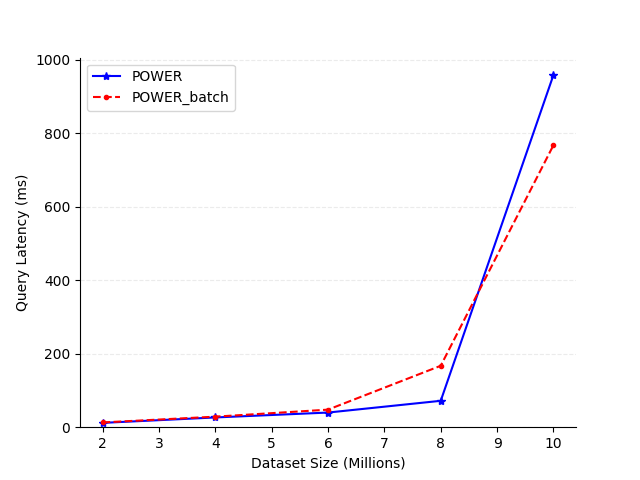
\includegraphics[width=0.4\textwidth]{../exp_plots/f_2-10m_50queries_20250314-222147.png}
    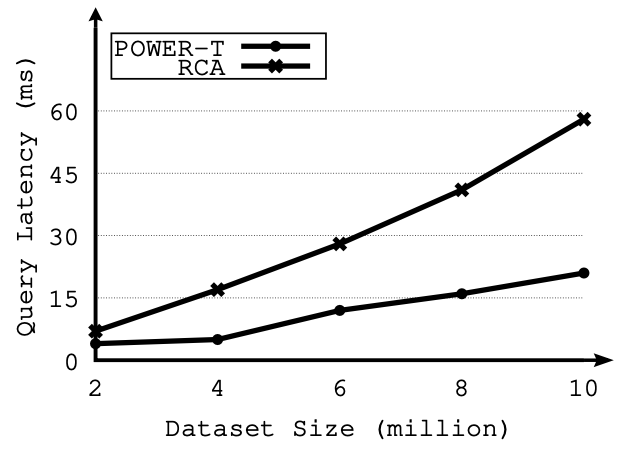
\includegraphics[width=0.4\textwidth]{./pics/paper-exp-f.png}
    \caption{Comparison of experiment f, left: our result, right: paper result}
\end{figure}

Comparing the left figure (our result) and the right figure (paper result), we can see that our version runtime is increasing exponentially with the dataset size while the paper version runtime is increasing linearly. We still need furthur investigation to find out the reason for this difference.

\section{Conclusion}

In this project, we have successfully replicated the experiments a, b, e, and f of the paper. The results of the experiments are similar to the paper results, but there are some differences in the runtime of the experiments. The differences may be due to the different hardwares and implementation languages, or a little bit implementation difference.

In this project, Mona and Kunyi have a tight cooperation from the understanding of the paper's content to the implementation and experiments. Kelvin also contributed to the paper reading and did his best to attempts the POWER\_batch algorithm. The project is a good opportunity for us to learn the spatial computing knowledge and improve our programming skills. We hope to have more opportunities to learn and practice in the future.

\newpage

\section*{Acknowledgements}
The authors wish to thank Professor Amr Magdy, Dr. Yongyi Liu, TA Alhassan Satii Alshareedah, and others who have helped us in this course for their valuable suggestions and patient guidance. Wish them all the best in their future work and life!

The contribution of each team member is as follows:

\begin{itemize}
\item Chou, Kelvin
\begin{itemize}
    \item Paper reading
    \item final report (appendix part)
    \item README.md
    \item Attempts of power\_batch.py (in ./Kelvin's src)
\end{itemize}

\item Yu, Kunyi
\begin{itemize}
    \item Paper reading
    \item Write the assignment3/5, final report
    \item Code decomposition
    \item Experiments implementation of a/b/e/f (provide 4 images of section 3)
\end{itemize}

\item Ibrahim, Mona
\begin{itemize}
    \item Paper reading
    \item Implemented the whole source code
          \begin{itemize}
              \item point.py
              \item quadTreeNode.py
              \item invertedIndex.py
              \item power.py
              \item power\_batch.py
              \item read\_data.py
              \item structured the queries
          \end{itemize}
    \item Experiments implementation of a/b/c (provide queries)
\end{itemize}
\end {itemize}

\begin{thebibliography}{10}
    \bibitem{ref1-original-paper} Liu, Yongyi, and Amr Magdy. "U-ASK: a unified architecture for kNN spatial-keyword queries supporting negative keyword predicates." Proceedings of the 30th International Conference on Advances in Geographic Information Systems. 2022.
    % \bibitem{ref2} 2
\end{thebibliography}

\section*{Appendix}

The following part is Kelvin's demonstration of his unfinished implementation for TKQN queries using the POWER algorithm:

\subsection*{Kelvin's Unfinished Implementation for TKQN Queries using POWER Algorithm}

\subsubsection*{Dataset Preparation}
The dataset comprises spatial objects defined by their coordinates  and associated keywords. Data preprocessing utilized Python's Pandas library for structured handling:

\begin{verbatim}
id,x,y,keywords
1,10,20,restaurant cafe
2,15,25,cafe bakery
3,20,30,restaurant bakery
\end{verbatim}

\subsubsection*{POWER Algorithm Implementation}
Due to constraints of the standard \texttt{rtree} Python library, a simplified brute-force method was implemented. This method evaluates keyword conditions and distances between query points and dataset objects directly:

\begin{verbatim}
def satisfies_keywords(keywords, positive, negative):
return positive.issubset(keywords) and negative.isdisjoint(keywords)

def distance(p1, p2):
return ((p1[0]-p2[0])**2 + (p1[1]-p2[1])**2)**0.5

def POWER_simple(query_location, positive, negative, k, data_objects):
results = []
for obj in data_objects:
if satisfies_keywords(obj['keywords'], positive, negative):
dist = distance(query_location, obj['location'])
heapq.heappush(results, (dist, obj))
return heapq.nsmallest(k, results)
\end{verbatim}

\subsubsection*{Batch Query Processing}
Batch query processing reduces redundant computations by executing multiple queries simultaneously:

\begin{verbatim}
def batch_POWER_simple(query_set, k, data_objects):
batch_results = {}
for qid, query in enumerate(query_set):
q_loc, positive, negative = query
results = POWER_simple(q_loc, positive, negative, k, data_objects)
batch_results[qid] = results
return batch_results
\end{verbatim}


\end{document}
